\section{Design}
\begin{figure}[H]
	\centering
	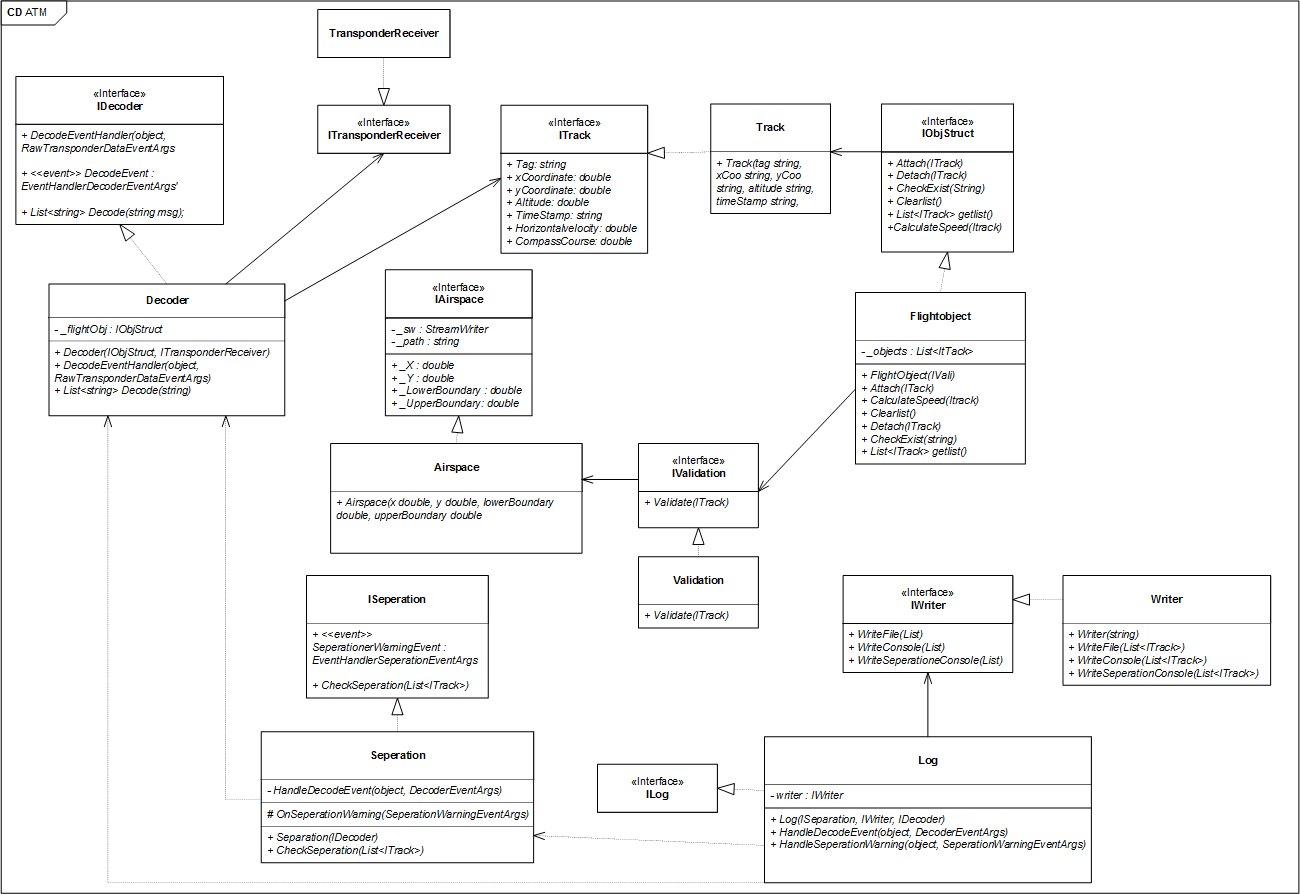
\includegraphics[width=1\linewidth]{../Diagrammer/CD_ATM_Fuld}
	\caption{CD over ATM}
	\label{fig:cdatm}
\end{figure}

\subsection{Decoder}
Decoder opgave er at tage imod beskeder fra Transreceiver. Derefter dele beskederne op i tag, X-koordinat, Y-koordinat, Altitude og Time. Dette data bruges til at oprette Tracks der indsættes i en objektstruktur
\subsection{Track}
Track opgave er at opdele en streng også oprette et nyt track som den tilfører et tag variable, X-koordinat variable, Y-koordinat variable, Altitude variable, Timestamp variable, Velocity variable og Compass course variable med henholdsvis den korrekte type. Denne her variable kan så opdateres ved brug af set metoden og dens specifikke variable kan tilgås ved hjælp af get.
\subsection{Flightobject}
Vores tracks bliver så lagt til en objektstruktur før den her objektstruktur lægger ind den given track, tager den og tjekker ved hjælp af validate funktionen om den given track er inden for vores airspace. Hvis den er i det given airspace tjekker den så om det givene track allerede er i objektstrukturen. Hvis den er det så opdatere den det given track for ikke at lave duplicate. Hvis den ikke er til stede i objektstrukturen så lægger den det given track ind i objektstrukturen. Hvis valideringen er udenfor airspace samtidig som den givne track er i vores liste. Betyder det at det givne fly har fløjet ud af vores airspace og skal dermed fjernes fra listen.
\subsection{Validation}
Validation tager et Airspace der har et defineret område. Dernæst har den en validate funktion der tager en ITrack ind som parameter. Dernæst bliver track elementets altitude sammenlignet med vores boundary værdier (lower boundary og upper boundary) samt at dens x-koordinat og y-koordinat er inden for airspacets bestemte x og y parameter. de her 3 tester er af typen bool validate returner så de her 3 resultater sammen med en AND operator som giver os true i det tilfælde at alle 3 testne er true og giver os false hvis kun en af dem er false. på den måde ved vi at hvis validate retunere true vil vores track som validate tager ind som parameter være inden for vores airspace
\subsection{Airspace}
Airspace definere vores boundary værdier for de områder hvor vi er interesseret i logføre alle fly. Måden det gøres på er at den tager en x og y størrelse, der definere den 2D udstrækning af vores airspace. Dernæst tager den også en lower boundary og upper boundary der definere vores 3D airspace. Lower boundary er fra jorden og til start højden af vores airspace. Upper boundary er højden på vores airspace. Vi kan tilgå airspacets størrelser ved hjælp af set og get funktioner.
\subsection{TransponderReceiver}
Vi får dataen fra alle fly der sender ud et transponder og bliver modtaget af en receiver. Den her data bliver så behandlet af vores decoder der afventer data gennem et event.
\subsection{Seperation}
Seperation tager ind en liste over alle fly der er i airspacet og tjekker x og y koordinater mod hinanden. Hvis den horisontale distance og vertikal distance er inden for et given område. Så sender den en seperation warning event.
\subsection{Log}
Log subscriber til seperation og decoder. Når der bliver sendt et event fra seperation skriver den så den data ind i en fil og dernæst til konsollen. Når den modtager et event fra decoder skriver den, den data ud til konsollen. 
\subsection{Writer}
Writer klassen står for at udskrive tekst ud til vores Konsol eller tekst til en fil. Konkret det den skriver ud er de tracks der er i vores airspace. Plus de tracks der er i seperation. De tracks der er i seperation skrives også til filen.

\begin{figure}[H]
	\centering
	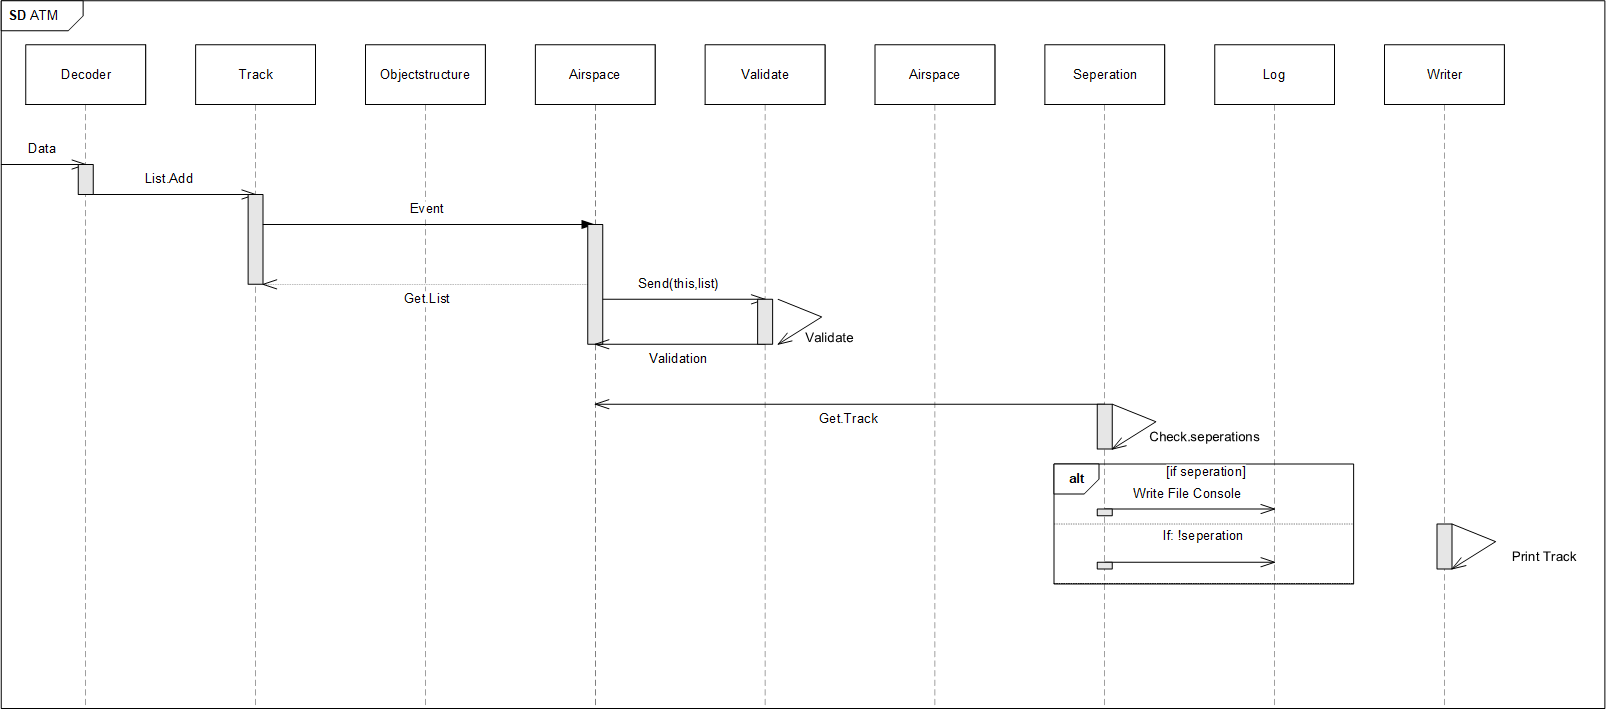
\includegraphics[width=1\linewidth]{../Diagrammer/SD_ATM}
	\caption{SD over ATM}
	\label{fig:sdatm}
\end{figure}

